\section{Parallel Results and Discussion}
\label{sec:parallel-results-and-discussion}

We demonstrate the strong and weak scaling of the current implementation. For each of the strong and weak scaling runs, we time the leaf and family callback stages for the build, upwards, and solve stages of the HPS method. This provides insight into the scalability of the leaf traversals as well as the family traversals for each stage.

For both strong and weak scaling analysis, we ran on the petascale machine Polaris at Argonne National Laboratory. Polaris is a 560 node machine, with each node consisting of one 2.8GHz AMD EPYC Milan 7543P 32 core CPU with 512 GB of DDR4 RAM.

\subsection{Strong Scaling}

Strong scaling analysis is done by solving a relatively large problem while increasing the number of compute units used to solve the problem. As one increases the parallelism, the compute per compute unit decreases at a rate equal to that at which the number of compute units is increasing. Ideal strong scaling should result in the time to solution decreasing at the same rate that the number of compute units is increasing.

Using the method of manufactured solutions, we generate a Poisson problem based on the exact solution
\begin{align}
    u_{\text{exact}}(x, y) = \sin(x) + \sin(y).
\end{align}
The resulting Poisson equation is thus
\begin{align}
    \nabla^2 u(x,y) = f(x,y) = -u_{\text{exact}}(x, y),
\end{align}
where the boundary conditions are provided by the exact solution. The leaf-indexed and path-indexed quadtrees that represent the underlying mesh are generated by recursively refining the root-level patch according to a refinement criteria of $|f(x,y)| > 1.2$. We used 8 levels of refinement, and patch sizes of $M = [8, 16, 32, 64]$. This results in solving the Poisson equation with an effective resolution of up to $8192 \times 8192$.

{\bf Results and Discussion}
The results of running on Polaris can be found in \reffig{fig:strong_scaling_plots}. For each patch size $M$ (indicated by the colors in \reffig{fig:strong_scaling_plots}), we increase the number of MPI ranks used to solve the problem. We show scaling on up to $N_R = 128$ MPI ranks.

\begin{figure}
    \centering
    \begin{tabular}{c}
        \begin{subfigure}[t]{0.95\textwidth}
            \centering
            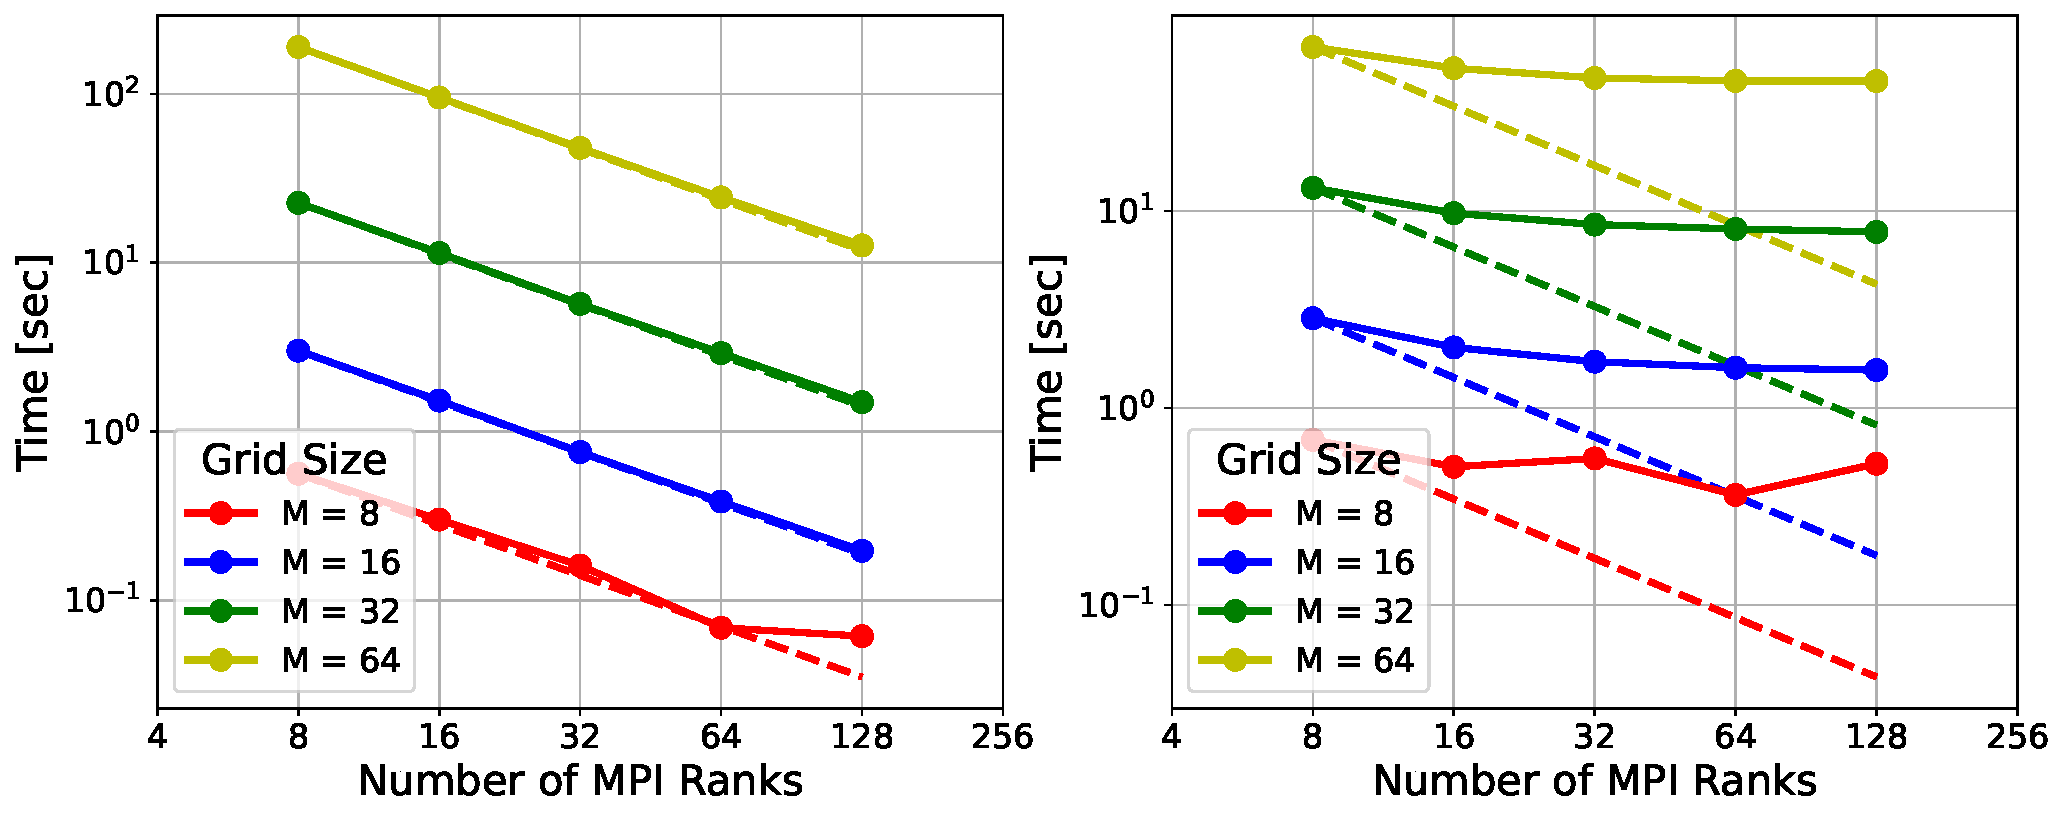
\includegraphics[width=\textwidth]{figures/build-strong-scaling-timing-no-title.pdf}
            \caption{The build stage strong scaling.}
            \label{subfig:strong_build}
        \end{subfigure}
        \\
        \begin{subfigure}[t]{0.95\textwidth}
            \centering
            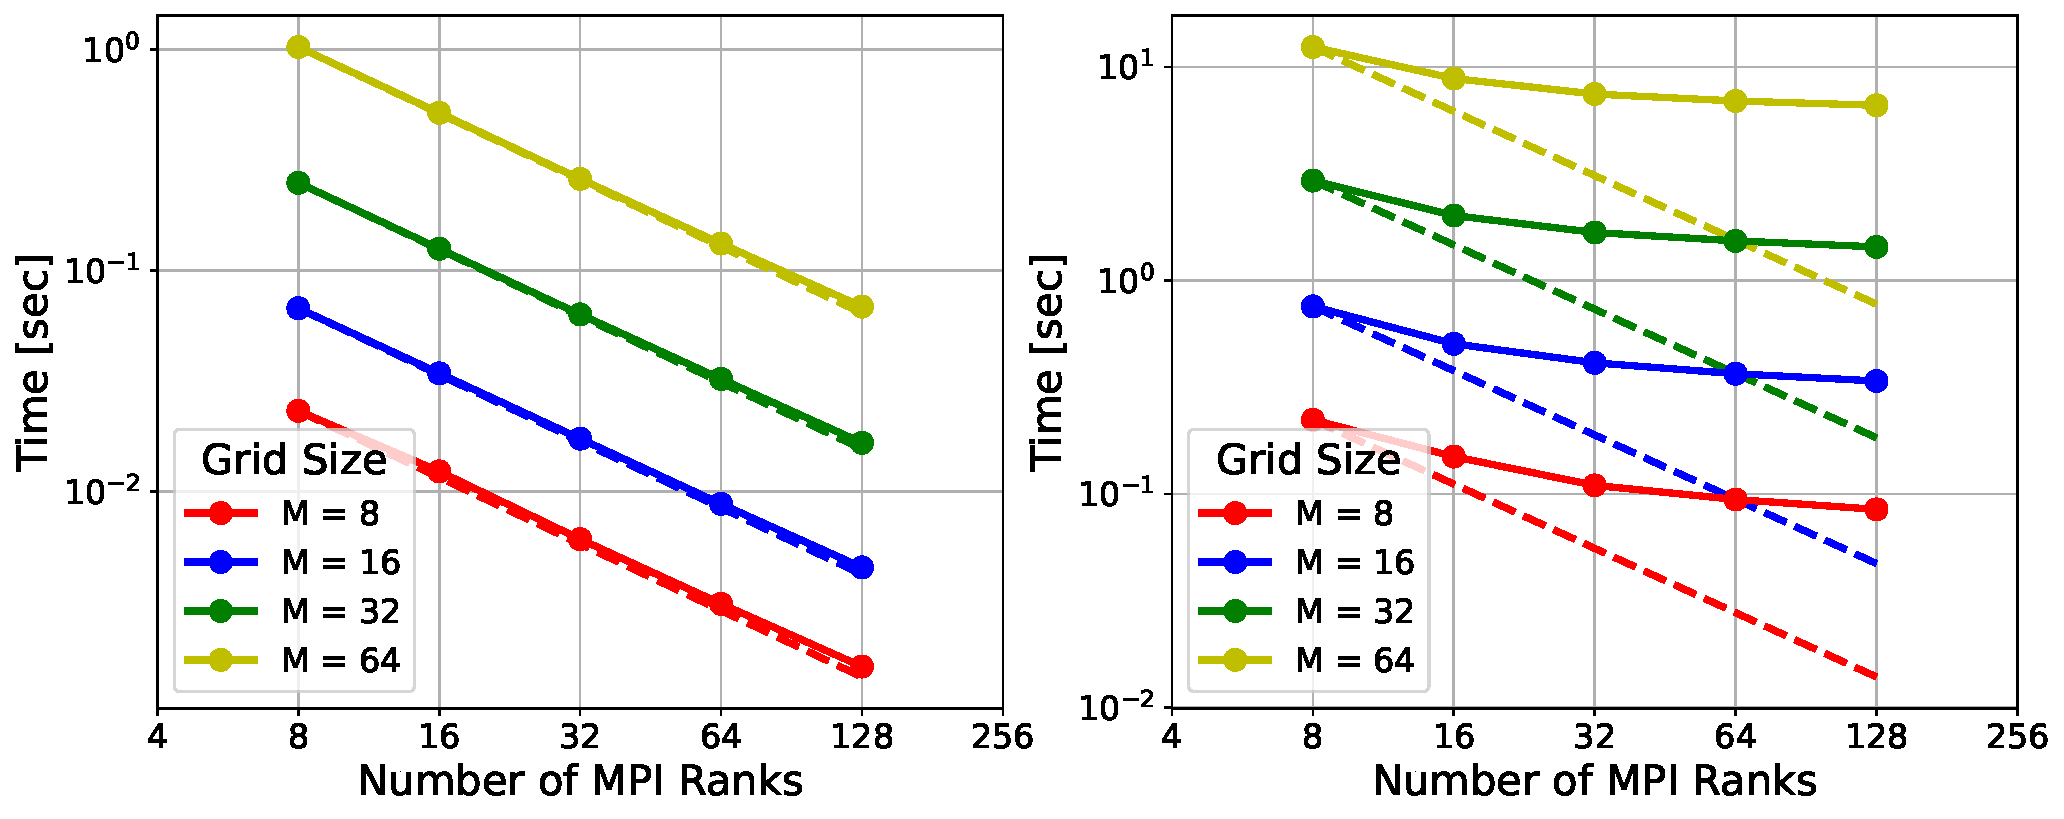
\includegraphics[width=\textwidth]{figures/upwards-strong-scaling-timing-no-title.pdf}
            \caption{The upwards stage strong scaling.}
            \label{subfig:strong_upwards}    
        \end{subfigure}
        \\
        \begin{subfigure}[t]{0.95\textwidth}
            \centering
            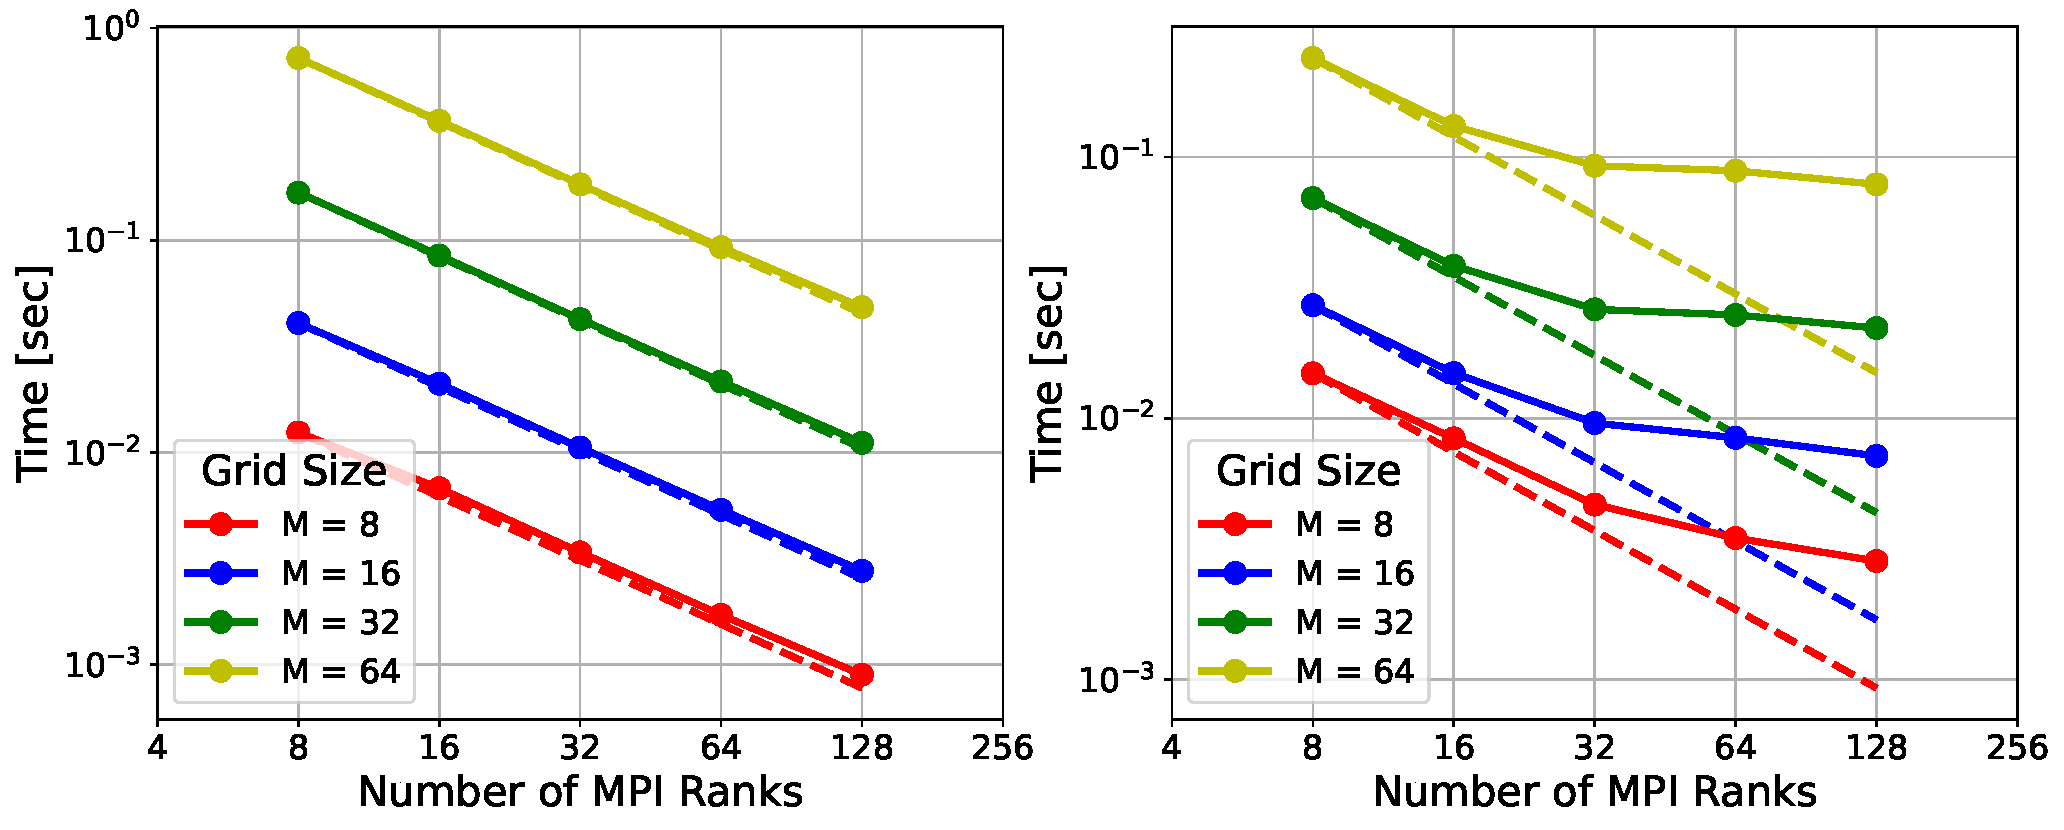
\includegraphics[width=\textwidth]{figures/solve-strong-scaling-timing-no-title.pdf}
            \caption{The solve stage strong scaling.}
            \label{subfig:strong_solve}
        \end{subfigure}
        \\
    \end{tabular}
    \caption{The strong scaling plots for the (a) build stage, (b) upwards stage, and (c) solve stage. For each, the left plot shows the scaling for the leaf callback and the right plot shows the scaling for the family callback. The solid line indicates actual timing and the dashed line indicates ideal strong scaling.}
    \label{fig:strong_scaling_plots}
\end{figure}

\reffig{fig:strong_scaling_plots} shows that the leaf callback functions for all three stages scale nearly perfectly. This is to be expected as there is no communication at this stage; each partition builds up the factorization or solves the elliptic problem independently. The family callbacks for all three stages have less than optimal scaling. In each stage, the family callback includes communicating data across families. Sibling nodes at intermediate levels (i.e., non-leaf nodes) are often owned by multiple ranks. The communication among ranks at the upper levels involves potentially global communication, including broadcast operations. This amount of communication is what leads to poor strong scaling at medium to larger runs; the amount of communication grows much faster than the compute time.

Comparing the strong scaling between the three different stages shows that the solve stage scales better than the build and the upwards stages. The size of the data involved in the communication in the solve stage is smaller than that in the factorization stages.

% \begin{figure}
%     \centering
%     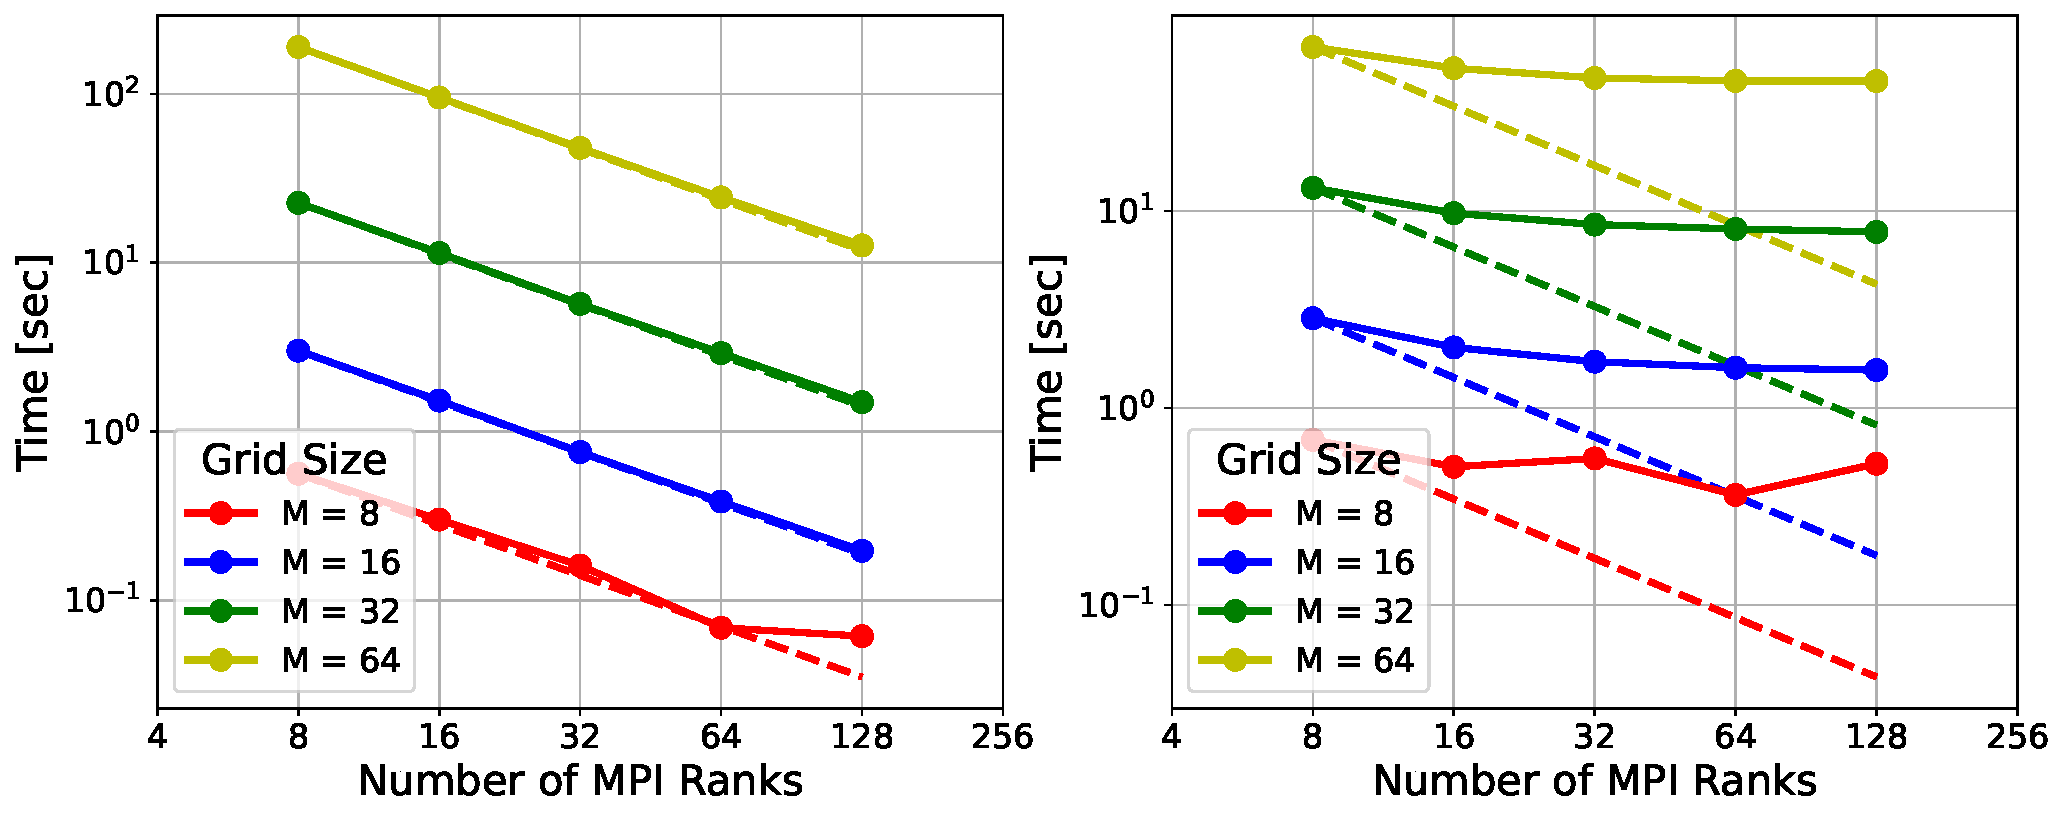
\includegraphics[width=\textwidth]{figures/build-strong-scaling-timing-no-title.pdf}
%     \caption{The strong scaling for the build stage. The left plot shows the scaling for the leaf callback and the right plot shows the scaling for the family callback. The solid line indicates actual timing and the dashed line indicates ideal strong scaling.}
%     \label{fig:strong_build}
% \end{figure}

% \begin{figure}
%     \centering
%     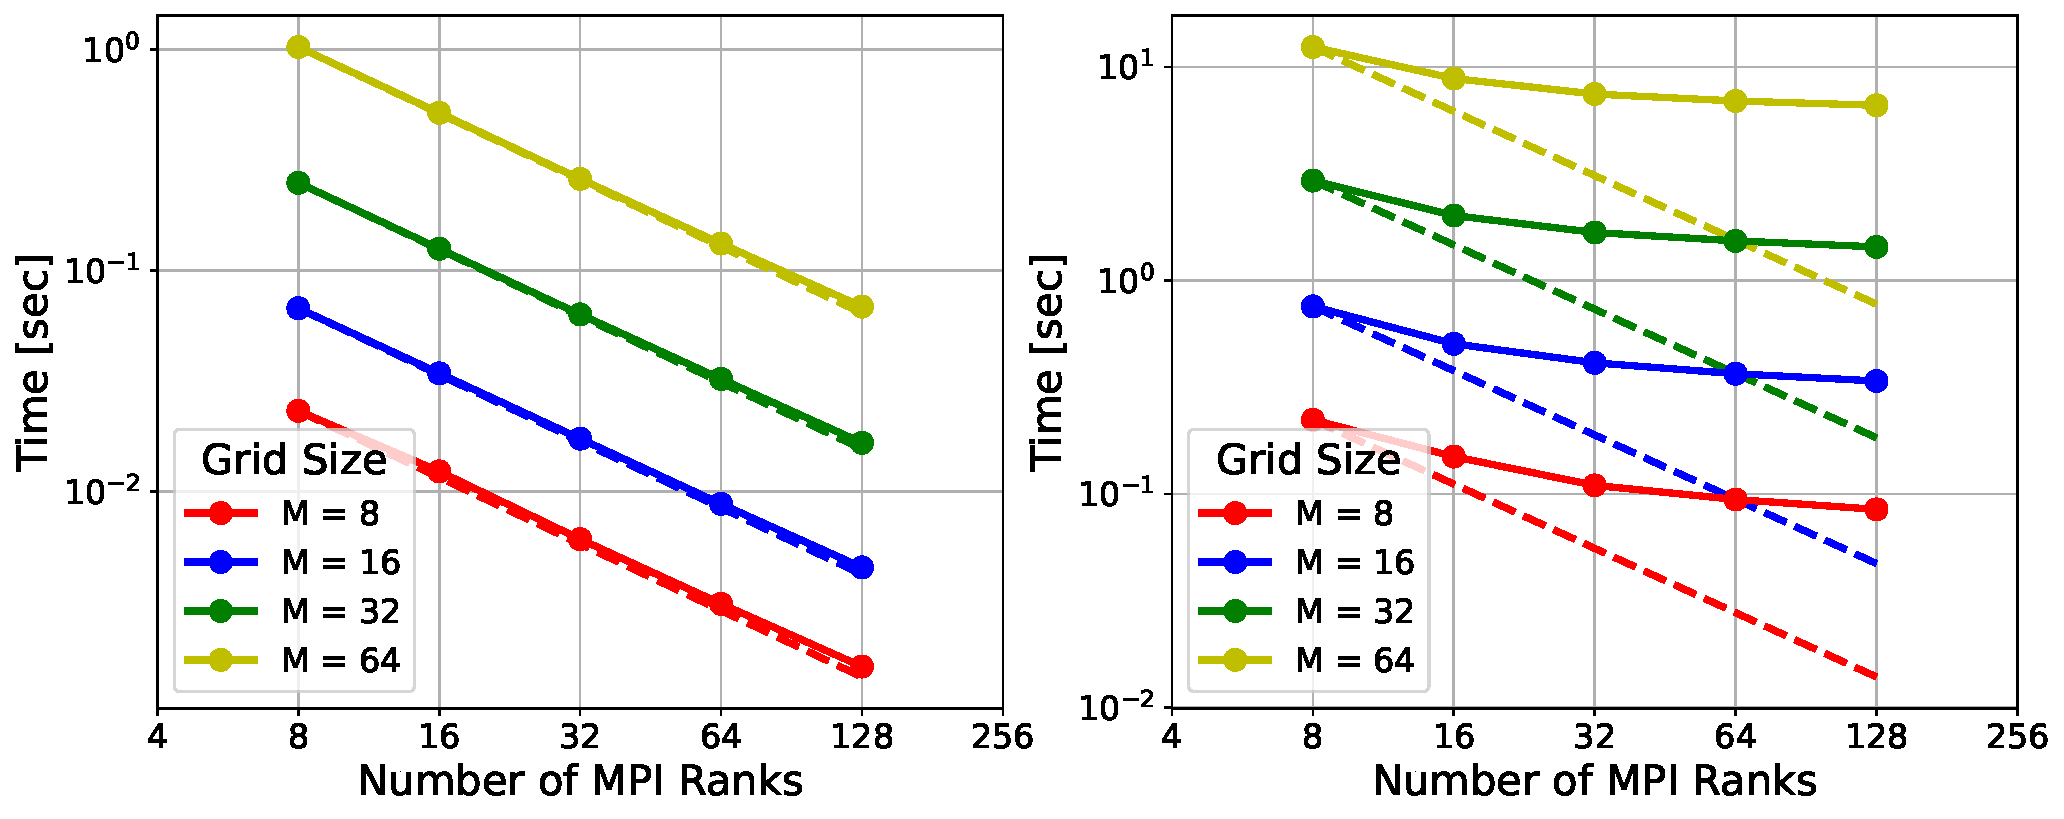
\includegraphics[width=\textwidth]{figures/upwards-strong-scaling-timing-no-title.pdf}
%     \caption{The strong scaling for the upwards stage. The left plot shows the scaling for the leaf callback and the right plot shows the scaling for the family callback. The solid line indicates actual timing and the dashed line indicates ideal strong scaling.}
%     \label{fig:strong_upwards}
% \end{figure}

% \begin{figure}
%     \centering
%     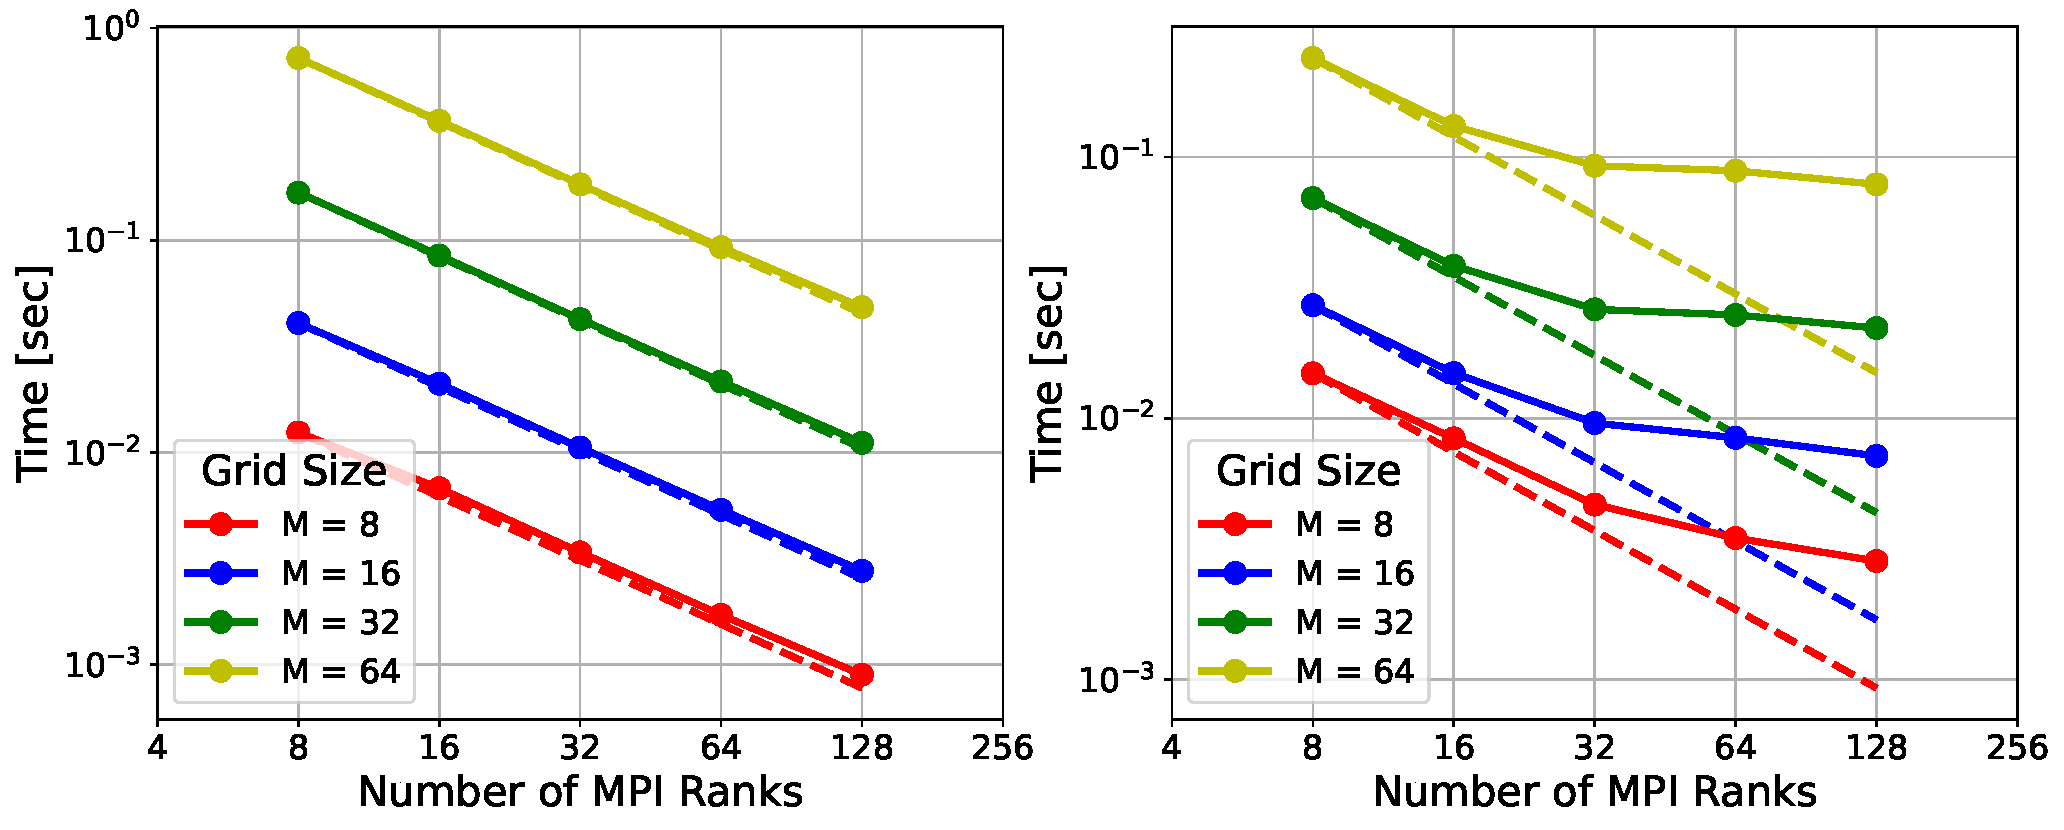
\includegraphics[width=\textwidth]{figures/solve-strong-scaling-timing-no-title.pdf}
%     \caption{The strong scaling for the solve stage. The left plot shows the scaling for the leaf callback and the right plot shows the scaling for the family callback. The solid line indicates actual timing and the dashed line indicates ideal strong scaling.}
%     \label{fig:strong_solve}
% \end{figure}

\subsection{Weak Scaling}
\label{sub:weak-scaling}

Weak scaling analysis is done by solving a problem while increasing both the size of the problem and the number of compute units. The compute time per compute unit stays constant in a weak scaling analysis and time to solution should stay constant as one increases the parallelism.

We solve the polar star Poisson problem with one polar star per compute unit (see \refsec{sub:example-two}). To keep the number of degrees of freedom constant per MPI rank, we solve on a square domain with a single polar star at the center. With each increase in the number of MPI ranks, we extend the domain to include more polar stars, each at the center of their own partition.

For this study, we refine around the edges of the polar stars. The refinement criteria was $|f(x,y)| > 1$, with 7 levels of refinement. Each polar star was a 4-pointed polar star with $r_0 = 0.3$, $r_1 = 0.4$, and $\epsilon = 0.015625$. We solve with patch sizes $M = [16, 32, 64]$, resulting in the degrees of freedom per MPI rank to be $[4096, 16384, 65536]$, respectively. An example of this setup can be found in \reffig{fig:polar-star-plots}, which shows the repeated solution and partitioning for $N_R = 4$ arranged in a $2 \times 2$ grid of processes.

\begin{figure}
    \centering
    \begin{tabular}{c c}
        \begin{subfigure}[t]{0.45\textwidth}
            \centering
            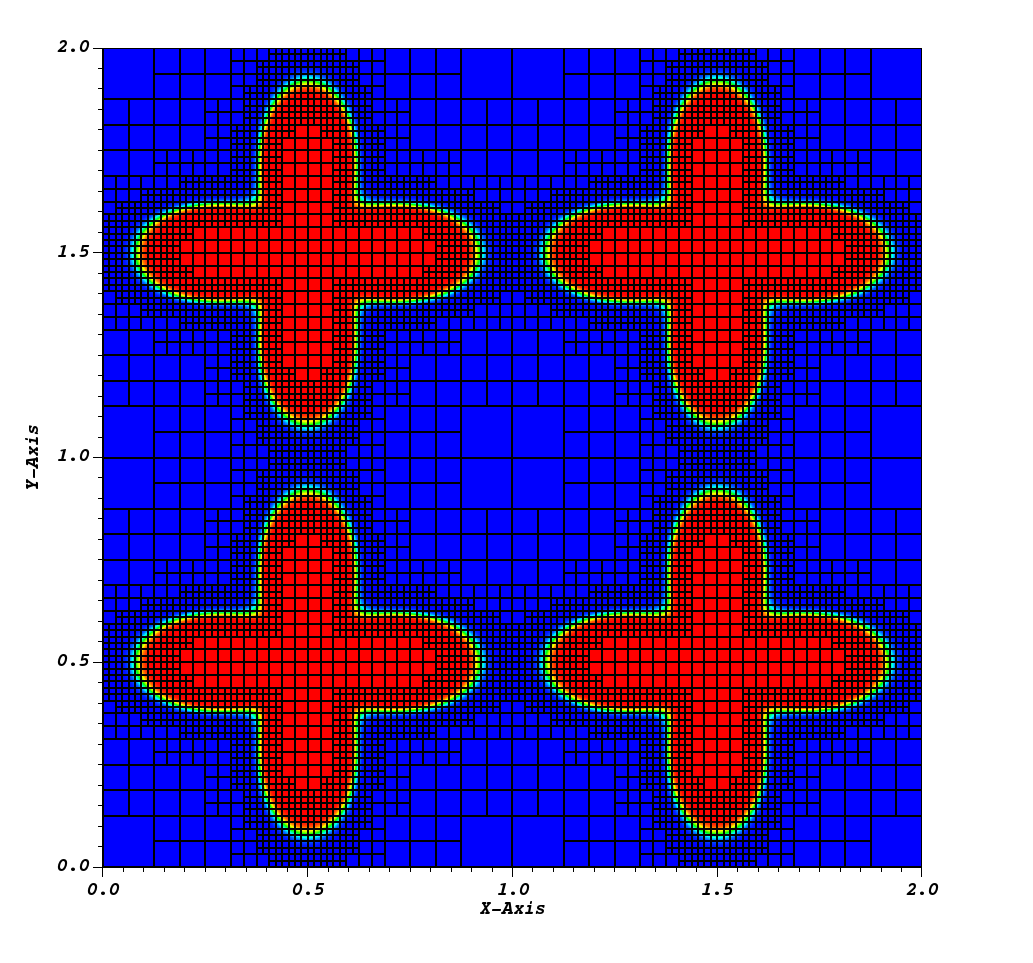
\includegraphics[width=\textwidth, clip=True, trim={0 0 0 0}]{figures/weak-scaling-stars.png}
            \caption{The plotted solution.}
            \label{subfig:polar-star-solution}
        \end{subfigure}
        &
        \begin{subfigure}[t]{0.45\textwidth}
            \centering
            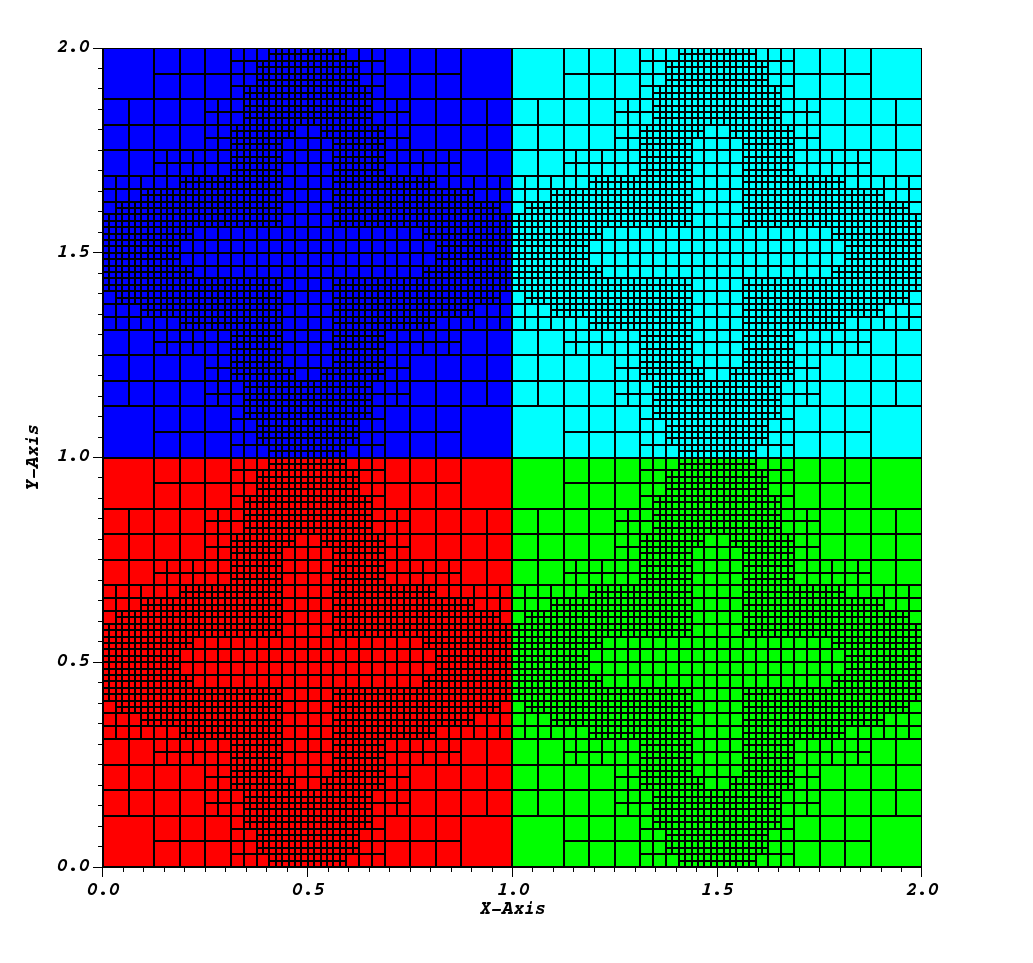
\includegraphics[width=\textwidth, clip=True, trim={0 0 0 0}]{figures/weak-scaling-partitions.png}
            \caption{The MPI partitions.}
            \label{subfig:polar-star-partitions}
        \end{subfigure}
    \end{tabular}
    \caption{Plots of the polar star Poisson problem used in the weak scaling study found in \refsec{sub:weak-scaling}. The polar star is generated from the RHS of the Poisson equation and is repeated for each MPI rank used to solve the problem. This shows four polar stars arranged in a $2 \times 2$ grid for solving with $N_R = 4$. Each outlined grid contains a $16 \times 16$ finite volume mesh.}
    \label{fig:polar-star-plots}
\end{figure}

{\bf Results and Discussion}
\reffig{fig:weak_scaling_plots} contains the results of the weak scaling runs. We plot the weak scaling efficiency, which is computed as
\begin{align}
    E_{\text{weak}} = \frac{t_{1}}{t_{N_R}} \times 100 \%,
\end{align}
where $t_{1}$ is the time spent in that stage on a single MPI rank. The colors indicate the different patch sizes, and the leaf and family callbacks are shown for all three stages.

Similarly to the strong scaling, the leaf callbacks scale better than the family callbacks. The build stage and solve stage leaf callbacks maintain nearly perfect weak scaling efficiency. The upwards stage scales similarly to the scaling of the family callbacks, which is unexpected. The family callbacks demonstrate similar scaling drop off as in the strong scaling. Again, this is likely due to the increased communication, along with the redundant calculations exhibited in this implementation.

\begin{figure}
    \centering
    \begin{tabular}{c}
        \begin{subfigure}[t]{0.95\textwidth}
            \centering
            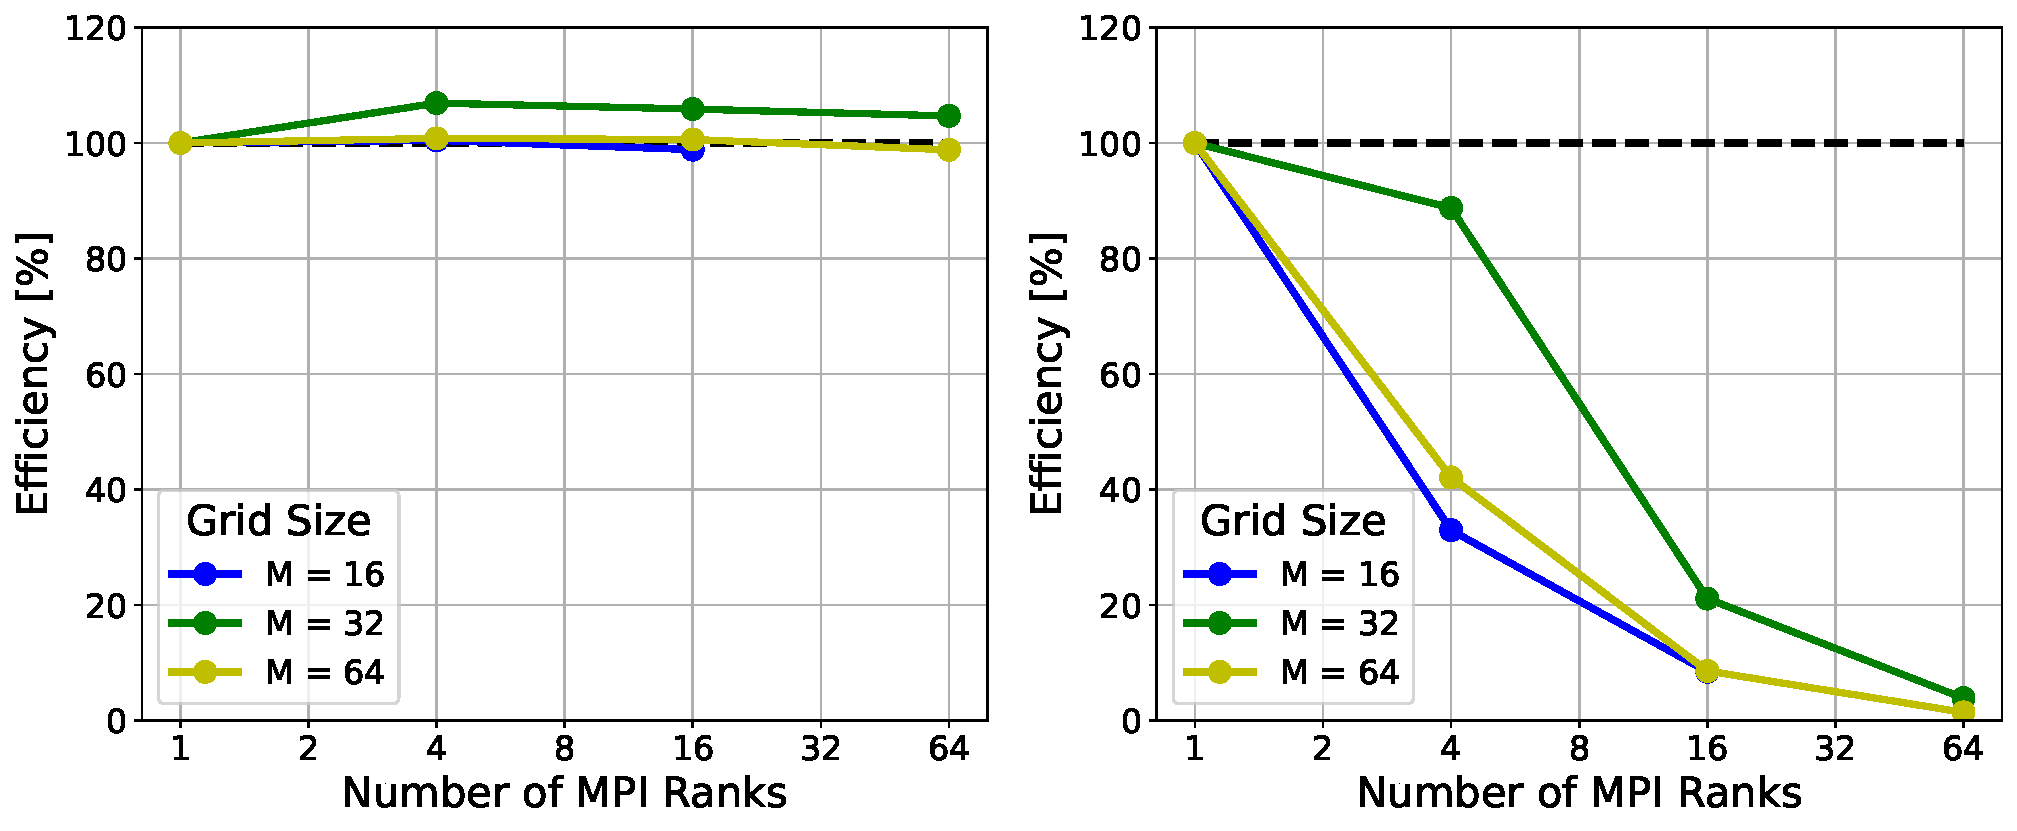
\includegraphics[width=\textwidth]{figures/build-weak-scaling-timing-no-title.pdf}
            \caption{The build stage weak scaling.}
            \label{subfig:weak_build}
        \end{subfigure}
        \\
        \begin{subfigure}[t]{0.95\textwidth}
            \centering
            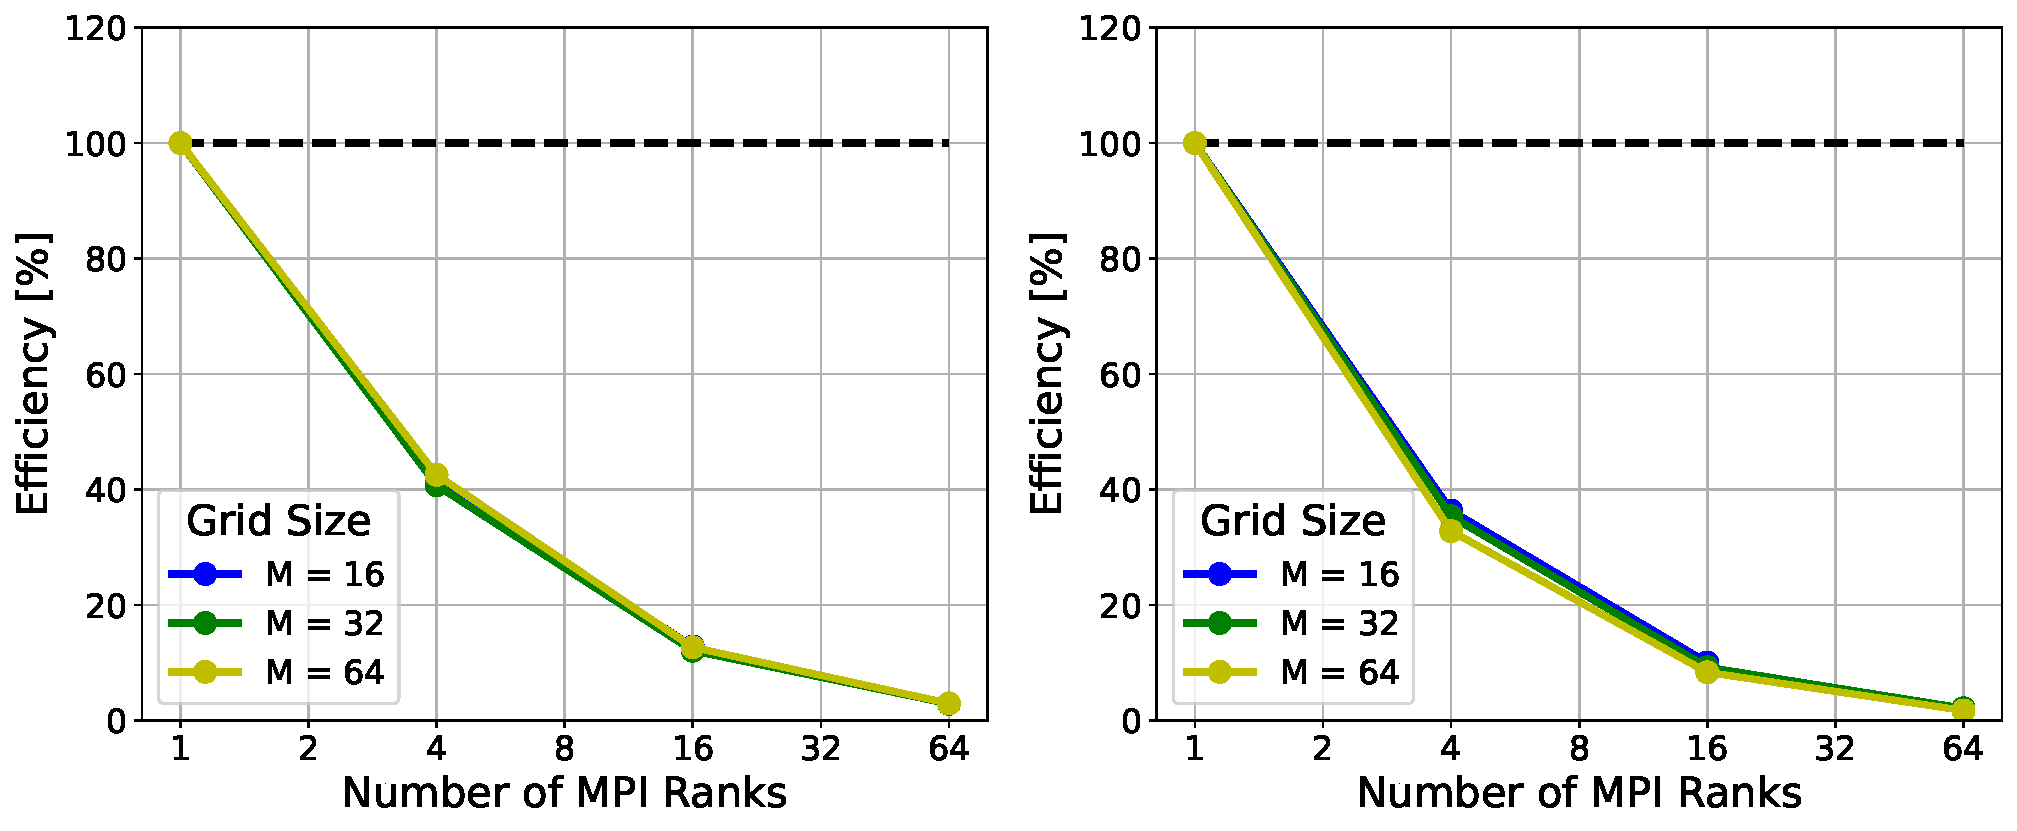
\includegraphics[width=\textwidth]{figures/upwards-weak-scaling-timing-no-title.pdf}
            \caption{The upwards stage weak scaling.}
            \label{subfig:weak_upwards}    
        \end{subfigure}
        \\
        \begin{subfigure}[t]{0.95\textwidth}
            \centering
            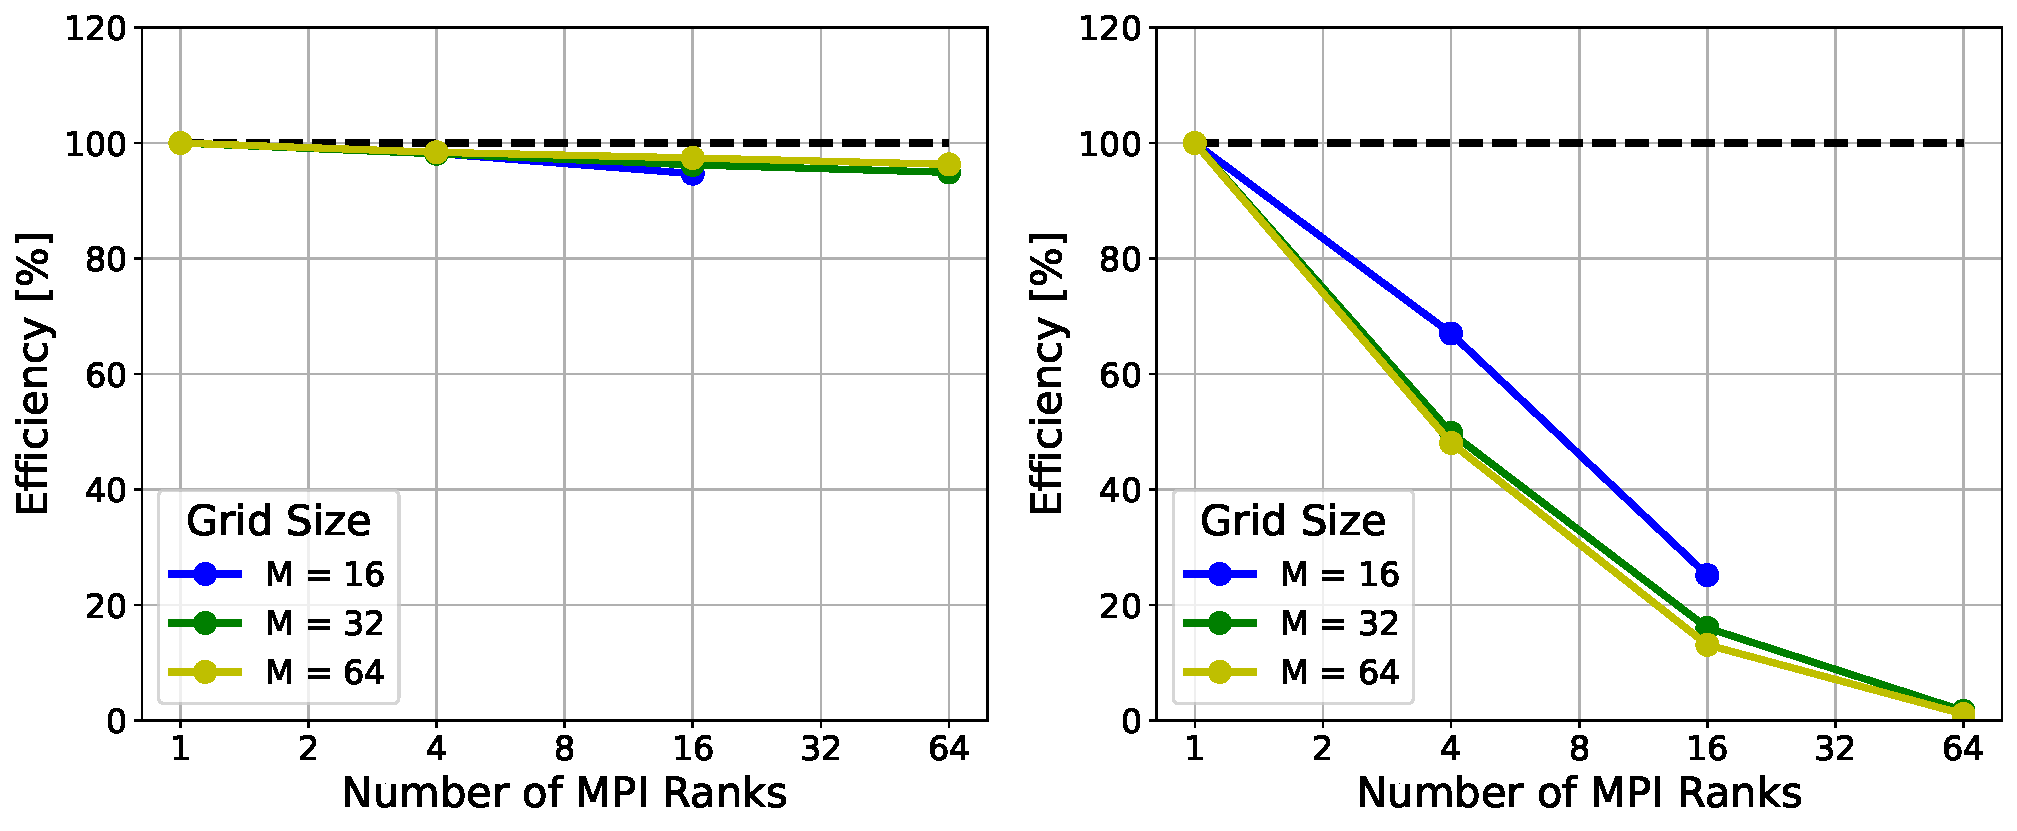
\includegraphics[width=\textwidth]{figures/solve-weak-scaling-timing-no-title.pdf}
            \caption{The solve stage weak scaling.}
            \label{subfig:weak_solve}
        \end{subfigure}
        \\
    \end{tabular}
    \caption{The weak scaling plots for the (a) build stage, (b) upwards stage, and (c) solve stage. For each, the left plot shows the scaling for the leaf callback and the right plot shows the scaling for the family callback. The solid line indicates actual efficiency and the dashed line indicates ideal weak scaling.}
    \label{fig:weak_scaling_plots}
\end{figure}

% \begin{figure}
%     \centering
%     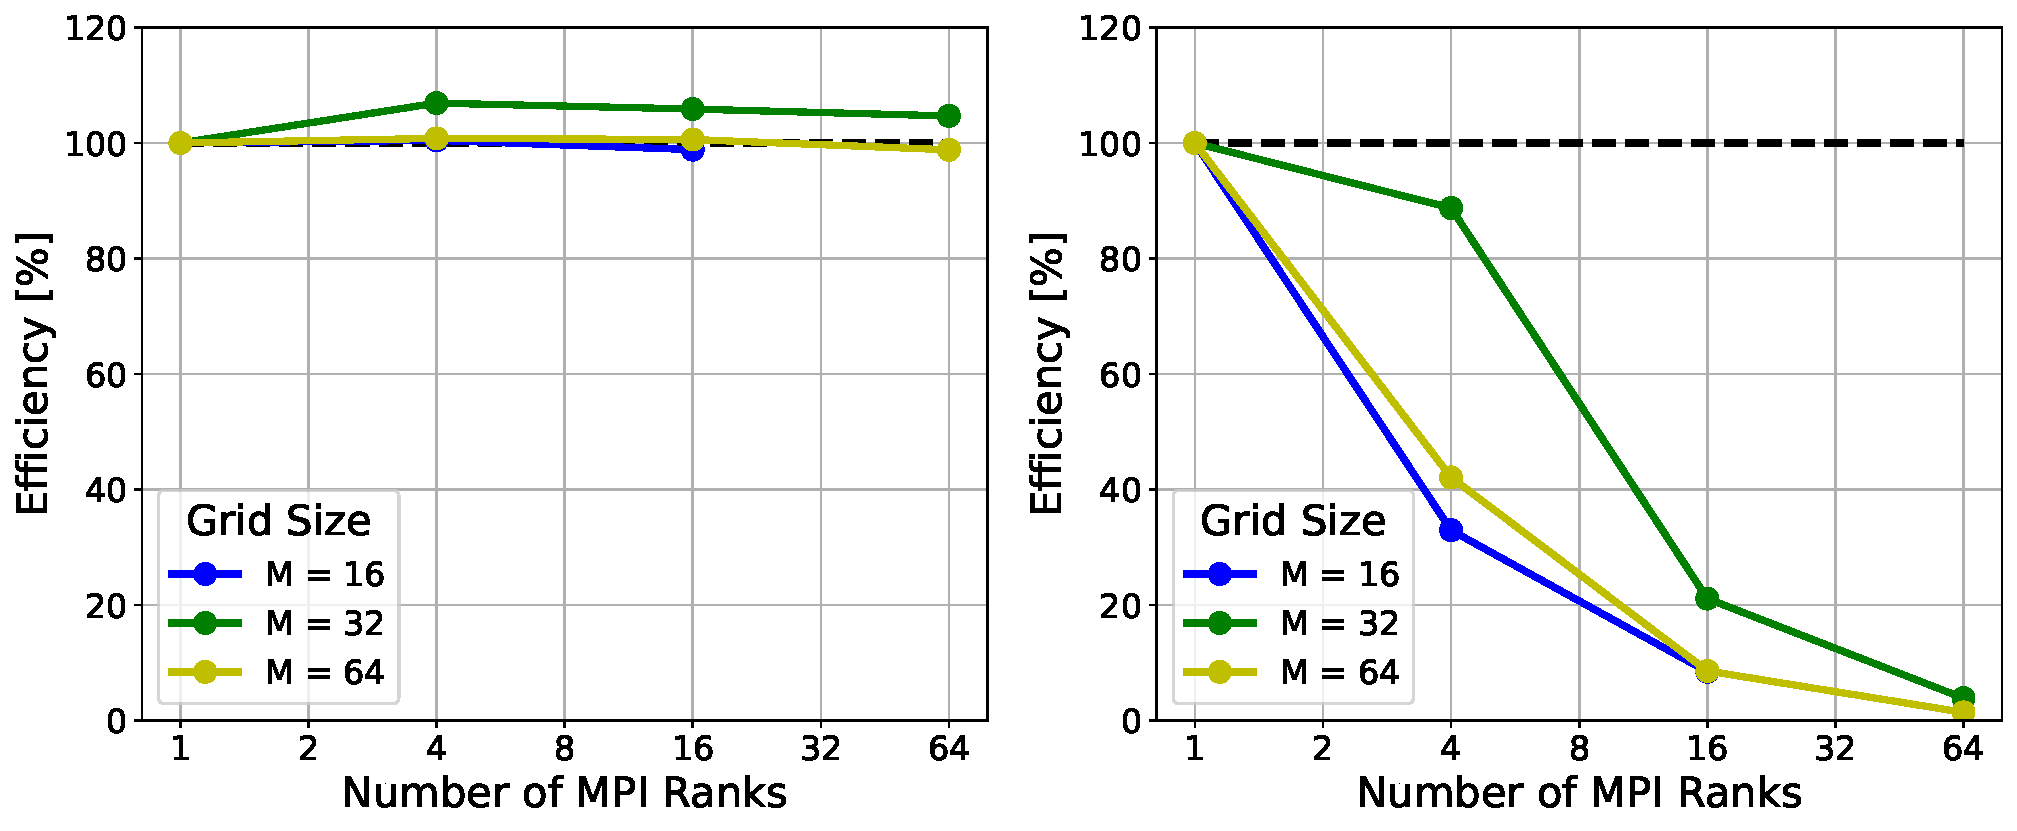
\includegraphics[width=\textwidth]{figures/build-weak-scaling-timing-no-title.pdf}
%     \caption{The weak scaling for the build stage. The left plot shows the scaling for the leaf callback and the right plot shows the scaling for the family callback. The solid line indicates actual timing and the dashed line indicates ideal weak scaling.}
%     \label{fig:weak_strong_build}
% \end{figure}

% \begin{figure}
%     \centering
%     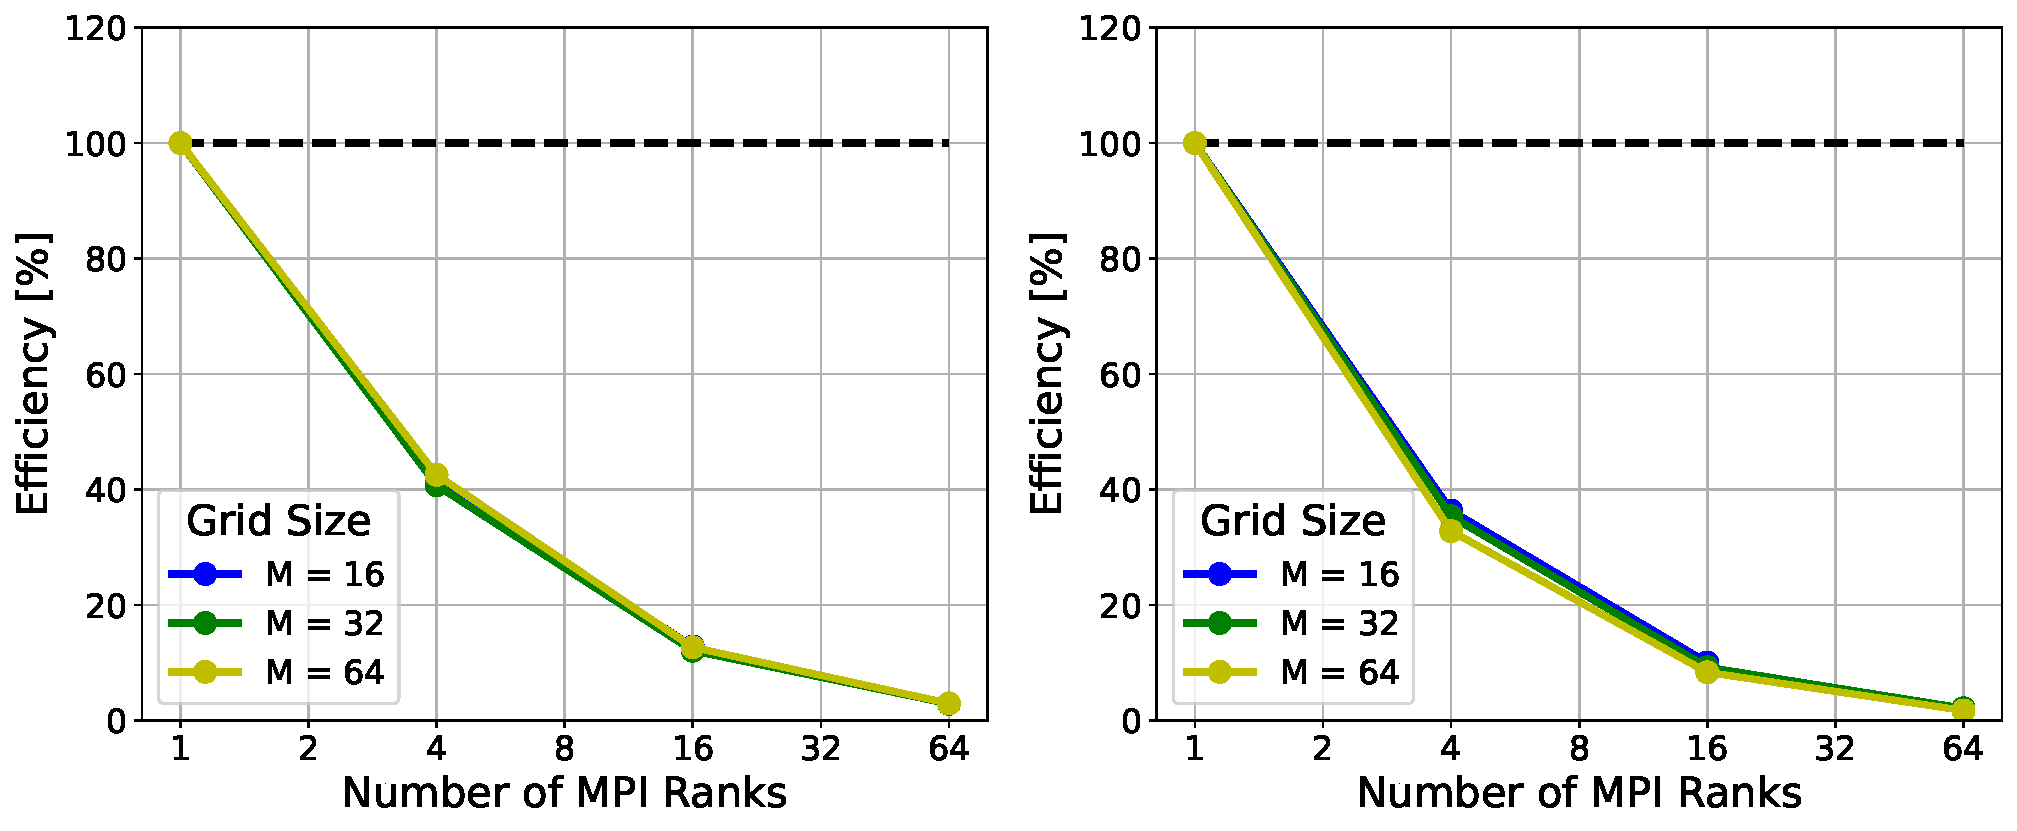
\includegraphics[width=\textwidth]{figures/upwards-weak-scaling-timing-no-title.pdf}
%     \caption{The weak scaling for the upwards stage. The left plot shows the scaling for the leaf callback and the right plot shows the scaling for the family callback. The solid line indicates actual timing and the dashed line indicates ideal weak scaling.}
%     \label{fig:weak_strong_upwards}
% \end{figure}

% \begin{figure}
%     \centering
%     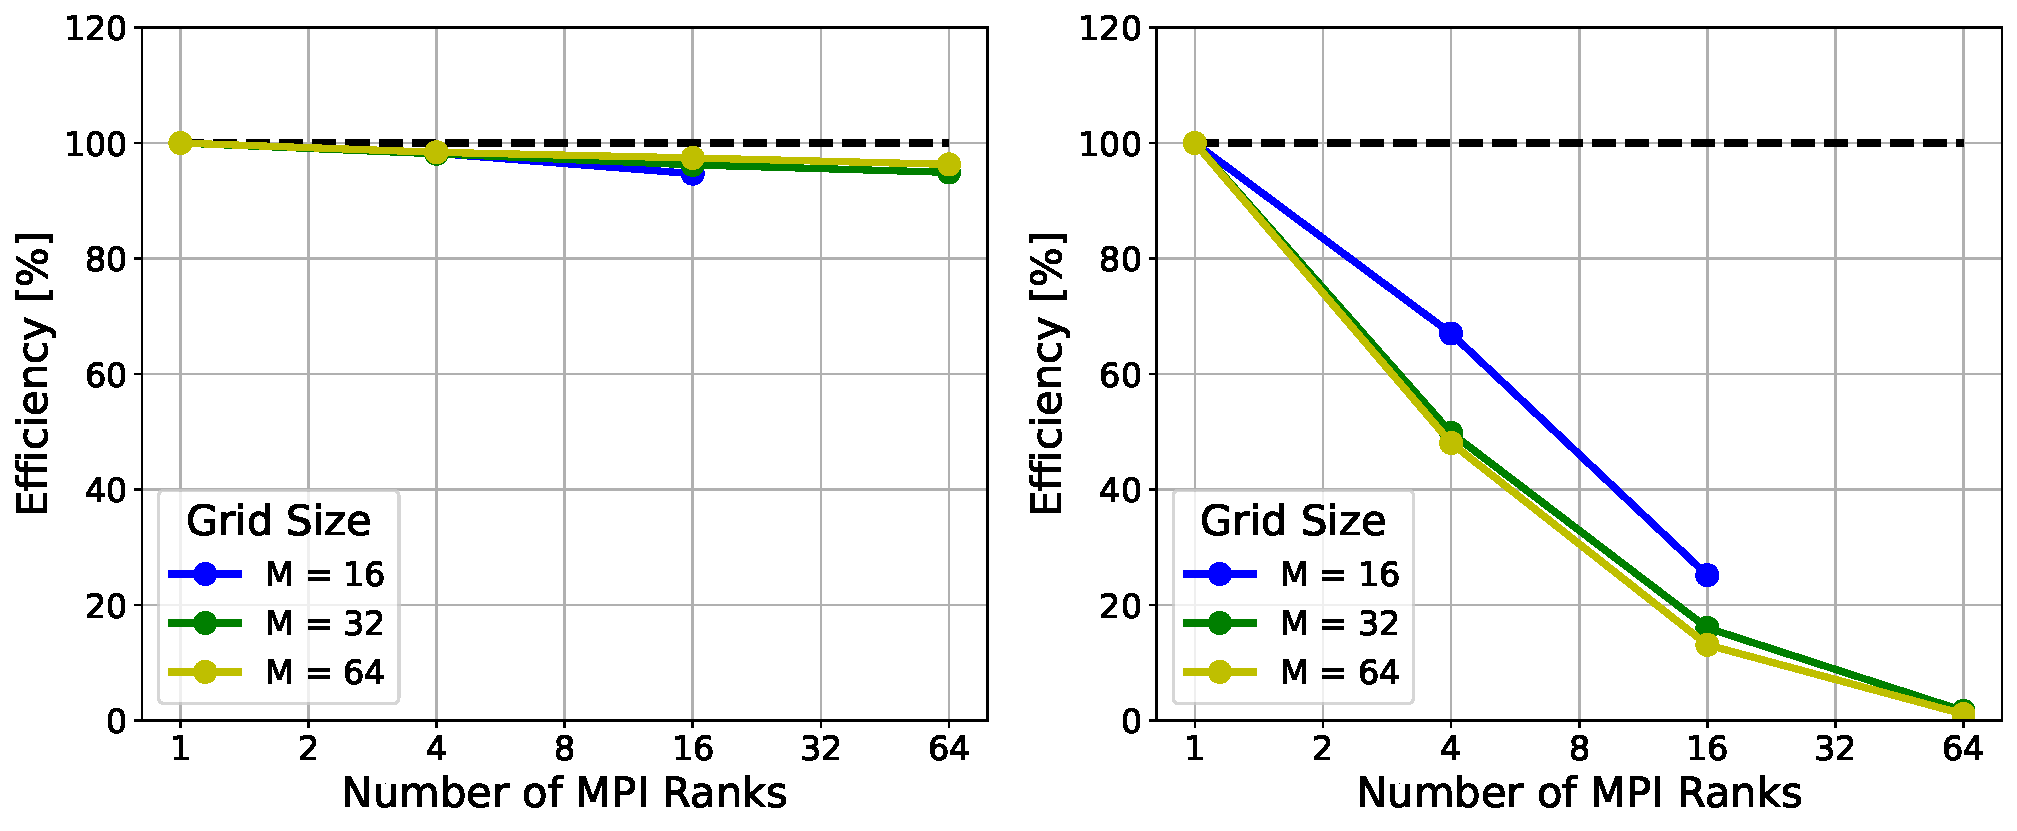
\includegraphics[width=\textwidth]{figures/solve-weak-scaling-timing-no-title.pdf}
%     \caption{The weak scaling for the solve stage. The left plot shows the scaling for the leaf callback and the right plot shows the scaling for the family callback. The solid line indicates actual timing and the dashed line indicates ideal weak scaling.}
%     \label{fig:weak_strong_solve}
% \end{figure}